\documentclass[tikz]{standalone}
\usepackage{pgfplots}
\pgfplotsset{compat=1.15}
\usepackage{mathrsfs}
\usetikzlibrary{arrows,calc}
\usepackage{tkz-euclide}
\pagestyle{empty}

\definecolor{AngleClr}{rgb}{0,0.39215686274509803,0}
\definecolor{ShapeClr}{rgb}{0.6,0.2,0}

\begin{document}

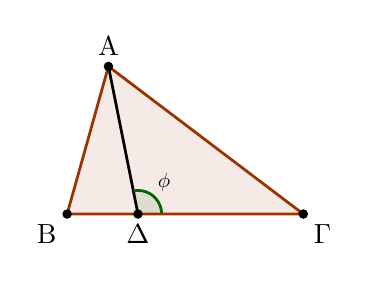
\begin{tikzpicture}[scale=.75]
\tkzSetUpLine[line width=1pt,color=black]
\tkzSetUpPoint[fill=black]

\tkzDefPoints{0/0/A,4/0/B,0.7/2.5/C,1.2/0/D}

\tkzFillPolygon[fill=ShapeClr,fill opacity=0.1,inner sep=1cm](A,B,C)

\tkzDrawSegment[line width=1pt,color=black](C,D)

\tkzFillAngle[fill=AngleClr,size=.4,fill opacity=0.1](B,D,C)
\tkzMarkAngle[line width=1pt,color=AngleClr,size=.4](B,D,C)
\tkzLabelAngle[pos=0.7](B,D,C){\scalebox{0.75}{$\phi$}}

\tkzDrawPolygon[color=ShapeClr](A,B,C)
\tkzDrawPoints[size=3](A,B,C,D)
\tkzLabelPoint[below left](A){$\rm B$}
\tkzLabelPoint[below right](B){$\rm \Gamma$}
\tkzLabelPoint[above](C){$\rm A$}
\tkzLabelPoint[below](D){$\rm \Delta$}

\end{tikzpicture}
\end{document}
